\documentclass[crop, tikz]{standalone}
\usetikzlibrary{positioning}
\usetikzlibrary{calc}
\begin{document}
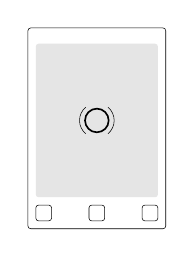
\begin{tikzpicture}[rounded corners=1, very thin]
    \newcommand\width{1.75}
    \newcommand\height{2.55}
    \newcommand\outborder{.1}
    \newcommand\button{2 * \outborder}

    \draw[fill=white] (0, 0) rectangle (\width, \height);

    \fill[black!10]
        (\outborder, 4 * \outborder) coordinate (screen-bl) rectangle
        (\width - \outborder, \height - 2 * \outborder) coordinate (screen-tr);

    \coordinate (screen-c) at ($(screen-bl)!.5!(screen-tr)$);

    \draw (\outborder, \outborder) rectangle
        ++(\button, \button);

    \draw (0.5 * \width - 0.5 * \button, \outborder) rectangle
        ++(\button, \button);

    \draw (\width - \outborder, \outborder) rectangle
        ++(-1 * \button, \button);

    \newcommand\innerradius{.15}
    \newcommand\outerradius{.22}
    \newcommand\partialangle{50}

    \draw[semithick] (screen-c) circle (\innerradius);

    \draw ($(screen-c)+(\outerradius, 0)$)
         arc[radius=\outerradius, start angle=0, delta angle=\partialangle]
         ($(screen-c)+(\outerradius, 0)$)
         arc[radius=\outerradius, start angle=0, delta angle=-\partialangle];

    \draw ($(screen-c)-(\outerradius, 0)$)
         arc[radius=\outerradius, start angle=180, delta angle=\partialangle]
         ($(screen-c)-(\outerradius, 0)$)
         arc[radius=\outerradius, start angle=180, delta angle=-\partialangle];
\end{tikzpicture}
\end{document}
